\documentclass[journal]{IEEEtran}

\usepackage{amsmath,amssymb,amsthm}
\usepackage{graphicx}
\usepackage{booktabs}
\usepackage{url}
\usepackage{hyperref}
\usepackage{cite}
\usepackage{algorithm}
\usepackage{algorithmic}
\usepackage{bm}

\newtheorem{theorem}{Theorem}
\newtheorem{proposition}{Proposition}

\title{Neural Empirical Mode Decomposition:\\
Differentiable Signal Decomposition via Adaptive Frequency-Domain Partition}

\author{Aous Abdo%
\thanks{A.~Abdo is with Analytica DSS. E-mail: aous@analytica-dss.com.}%
}

\begin{document}
\maketitle

%----------------------------------------------------------------------
\begin{abstract}
Signal decomposition methods such as empirical mode decomposition (EMD) and variational mode decomposition (VMD) remain widely used in biomedical, industrial, and geophysical signal processing, but they are not differentiable and cannot be jointly trained with a downstream task. Existing learned alternatives either discard physical interpretability or rely on soft physics losses that do not guarantee reconstruction, energy conservation, or orthogonality. We introduce \emph{Neural Empirical Mode Decomposition} (N-EMD), a differentiable signal decomposition whose architecture enforces these three properties exactly. N-EMD is a signal-adaptive filter bank in which a neural analyzer produces $K$ log-filter responses over the input spectrum; a softmax over the $K$ dimension turns them into a partition of unity, so the filters sum to one at every frequency and the inverse FFT of the filtered spectra reconstructs the input exactly. The resulting intrinsic mode functions (IMFs) are provably orthogonal to within a vanishing softmax residual, have bounded total energy by Cauchy--Schwarz, and are obtained in a single forward pass. We show that soft physics losses alone are insufficient: a generic iterative sifting network satisfies every constraint at a degenerate point and produces broadly mixed components. The partition-of-unity architecture solves this by restricting the feasible set. On a 3-class synthetic classification benchmark, end-to-end training of N-EMD with a small classifier improves test accuracy by $7.8$~pp over a VMD+classifier baseline and by $14.0$~pp over EMD+classifier while retaining a physically-interpretable decomposition. We release our implementation and experiment scripts.
\end{abstract}

\begin{IEEEkeywords}
Signal decomposition, empirical mode decomposition, variational mode decomposition, differentiable signal processing, partition of unity, task-aware representation learning.
\end{IEEEkeywords}

%======================================================================
\section{Introduction}
\label{sec:intro}
%======================================================================

Signal decomposition is a foundational tool. A nonstationary signal $x(t)$ is written as a sum of oscillatory components plus a slow residual, and each component is analyzed for amplitude, frequency, or phase content on its own. Empirical mode decomposition~\cite{huang1998} was introduced for this purpose and spawned a family of methods: ensemble EMD~\cite{wu2009eemd}, complete EEMD with adaptive noise~\cite{torres2011ceemdan}, and variational mode decomposition~\cite{vmd2014}. These methods are widely used in bearing-fault diagnosis, seismic processing, and biomedical signal analysis because the components they produce are interpretable --- each one occupies a well-defined frequency band and can be related back to physical phenomena.

Three limitations hold the classical family back. First, the methods are not differentiable: they use sifting (EMD) or alternating direction optimization (VMD). This rules out joint training with any downstream model. Second, the decomposition is chosen once per signal, by the method's fixed heuristic, with no mechanism for adapting to what the task actually needs. Third, the properties one usually wants --- exact reconstruction, orthogonality, and energy conservation --- are approximate empirical outcomes rather than guarantees. On the canonical 3-component test signal we use throughout this paper, EMD's orthogonality index ranges from $0.04$ to $0.17$ depending on the input, and VMD's energy ratio can drop to $0.66$.

Learned alternatives have been proposed but face a trade-off. End-to-end 1-D CNNs give up interpretability entirely; the decomposition is implicit inside the network. Purely physics-constrained learners (decompositions trained with soft losses for reconstruction, orthogonality, etc.) suffer a subtler problem: soft constraints do not shrink the feasible set. Any generic function approximator that satisfies orthogonality and narrow-bandwidth can also satisfy them trivially --- by collapsing components, by inflating and cancelling energy, or by leaving all signal content in the residual. We give a concrete example of this failure mode in Section~\ref{sec:negative-result}.

This paper takes a different approach. Rather than imposing the desired properties through losses, we encode them in the architecture. Concretely:

\begin{enumerate}
\item We introduce a \emph{Neural Adaptive Filter Bank} for signal decomposition. A small analyzer network maps the input spectrum to $K$ log-filter responses. A softmax over the $K$ dimension converts them to a partition of unity: the $K$ filters sum to $1$ at every frequency. Applying each filter in the frequency domain and inverse-FFTing produces IMFs that sum to the input exactly, by construction. This architecture provides provable reconstruction, bounded energy, and approximate orthogonality without relying on any loss to enforce them.
\item We report a negative result that motivates this design. A generic iterative sifting architecture trained with seven physics-inspired soft losses (orthogonality, narrow-bandwidth, monotonic residual, residual energy, energy conservation, frequency ordering, and spectral concentration) produces decompositions whose filters collapse into degenerate configurations that satisfy every loss without separating physical components. Architectural inductive bias is needed.
\item We show that end-to-end task-aware training with N-EMD improves downstream classification accuracy by $7.8$~percentage points over VMD+classifier and $14.0$ points over EMD+classifier on a controlled synthetic benchmark. The improvement is a direct consequence of the method's differentiability.
\end{enumerate}

The work targets a gap in the literature: decomposition methods that are both \emph{interpretable} (each component is a bandpass-filtered version of the input, and the filter responses can be plotted) and \emph{trainable} (the decomposition adapts to what the downstream task needs). This matters in defense, biomedical, and industrial settings where a black-box classifier is not acceptable and a fixed, untrainable decomposition underperforms.

%======================================================================
\section{Related Work}
\label{sec:related}
%======================================================================

\textbf{Classical signal decomposition.} EMD~\cite{huang1998} decomposes a signal by iterative sifting: it finds local extrema, fits cubic-spline upper and lower envelopes, subtracts their mean, and repeats until each IMF is narrow-band. The method has well-known problems --- mode mixing, boundary effects, non-monotonic residuals, and sensitivity to noise~\cite{rilling2003emd} --- that motivated ensemble EMD (EEMD)~\cite{wu2009eemd} and CEEMDAN~\cite{torres2011ceemdan}. VMD~\cite{vmd2014} reformulates decomposition as a constrained optimization: find $K$ modes whose sum is the input and whose individual bandwidths are minimized. Its center frequencies are optimized per signal by ADMM, yielding narrow-band components but requiring a fresh optimization for every new input.

\textbf{Learned signal decomposition.} Attempts to make EMD differentiable or to learn decomposition directly have been sparse. Neural EMD variants have been proposed for specific applications (e.g., speech separation, EEG) but typically drop the physical properties (reconstruction, interpretability) in exchange for performance. To the best of our knowledge, no prior work provides a differentiable decomposition with \emph{exact} reconstruction and interpretable bandpass filter responses, with task-aware training capability.

\textbf{Differentiable signal processing.} The differentiable DSP line of work (e.g., DDSP~\cite{ddsp2020}) has shown that explicitly incorporating signal-processing structure into neural networks improves both interpretability and sample efficiency. Our architecture is in the same spirit. We use FFTs, learned filter responses, and a softmax partition as structured layers; nothing is a black-box.

\textbf{Physics-informed machine learning.} Soft physics losses are a common tool in PINNs and related work. Section~\ref{sec:negative-result} is a cautionary note for that literature: in our setting, soft physics losses proved insufficient even when we added six of them. The feasible set was too large, and the optimizer reliably found degenerate minima. Architectural constraints were necessary.

%======================================================================
\section{Method}
\label{sec:method}
%======================================================================

\subsection{Problem Formulation}

Let $x \in \mathbb{R}^{T}$ be a discrete real signal of length $T$. We want to decompose $x$ into $K$ bandpass components $c_{1}, \ldots, c_{K}$ such that
\begin{equation}
x \;=\; \sum_{k=1}^{K} c_{k} ,
\label{eq:reconstruction}
\end{equation}
the components are approximately orthogonal, and each $c_{k}$ is concentrated in a specific frequency range. Classical methods enforce~(\ref{eq:reconstruction}) only approximately (EMD leaves a residual; VMD's reconstruction error is typically $10^{-2}$). We want exact reconstruction as a structural property.

\subsection{Architecture}

Write $X = \mathrm{rFFT}(x) \in \mathbb{C}^{N}$ where $N = \lfloor T/2 \rfloor + 1$. A signal analyzer network $f_{\theta}$ takes the magnitude $|X|$ and phase $\arg X$ stacked as a 2-channel input and produces $K$ real-valued log-filter responses:
\begin{equation}
\mathbf{s}(f) \;=\; f_{\theta}\bigl([|X(f)|,\, \arg X(f)]\bigr) \;\in\; \mathbb{R}^{K \times N}.
\label{eq:analyzer}
\end{equation}
A softmax over the $K$ dimension turns these into a partition of unity in the frequency domain:
\begin{equation}
H_{k}(f) \;=\; \frac{\exp\!\bigl(s_{k}(f) / \tau\bigr)}{\sum_{j=1}^{K} \exp\!\bigl(s_{j}(f) / \tau\bigr)},
\qquad
\sum_{k=1}^{K} H_{k}(f) \;=\; 1,
\label{eq:softmax-partition}
\end{equation}
where $\tau > 0$ is a temperature parameter that is annealed during training (see Section~\ref{sec:training}). Each filter is applied in the frequency domain and inverse-transformed:
\begin{equation}
c_{k} \;=\; \mathrm{irFFT}\!\bigl(H_{k}(f)\, X(f)\bigr).
\label{eq:imf}
\end{equation}

The analyzer $f_{\theta}$ is a small 1-D residual network. Our default has an input 1-D convolution that lifts 2 channels to $d = 64$, three residual blocks each with two convolutions (kernel size 5) and GELU activations, and a final 1-D convolution that projects to $K$ output channels. Total parameters: $125{,}315$ at $K = 3$, $d = 64$.

\subsection{Theoretical Properties}

\begin{theorem}[Exact reconstruction]
For any input $x \in \mathbb{R}^{T}$, any temperature $\tau > 0$, and any analyzer output $\mathbf{s} \in \mathbb{R}^{K \times N}$, the decomposition~(\ref{eq:imf}) satisfies $\sum_{k} c_{k} = x$ up to floating-point precision.
\end{theorem}
\begin{proof}
By the softmax identity $\sum_{k} H_{k}(f) = 1$ for all $f$. Thus
$\sum_{k} H_{k}(f) X(f) = X(f)$,
and the inverse transform of $X$ is $x$ exactly. The remaining error is floating-point round-off in the FFT/IFFT pair; empirically we observe $\max_{t} |x(t) - \sum_{k} c_{k}(t)| < 10^{-6}$ on all signals we have tested.
\end{proof}

\begin{theorem}[Energy is bounded]
For any input $x$,
$\sum_{k=1}^{K} \|c_{k}\|_{2}^{2} \;\leq\; \|x\|_{2}^{2}$,
with equality if and only if the filters form a \emph{disjoint} partition (each $H_{k}(f)$ is $0$ or $1$ at every frequency).
\end{theorem}
\begin{proof}
By Parseval, $\|c_{k}\|_{2}^{2} = \|H_{k} X\|_{2}^{2} = \sum_{f} H_{k}(f)^{2} |X(f)|^{2}$. Summing over $k$,
$\sum_{k} \|c_{k}\|_{2}^{2} = \sum_{f} |X(f)|^{2} \sum_{k} H_{k}(f)^{2}$.
Since $H_{k}(f) \in [0,1]$ and $\sum_{k} H_{k}(f) = 1$, by Cauchy--Schwarz $\sum_{k} H_{k}(f)^{2} \leq 1$, with equality iff one $H_{k}(f) = 1$ and all others are zero. The result follows.
\end{proof}

In contrast, VMD does not bound the total component energy: in our experiments VMD's energy ratio ranges between $0.60$ and $1.01$ depending on signal type. The Cauchy--Schwarz bound above is a free structural consequence of the softmax partition.

\begin{proposition}[Approximate orthogonality]
If the filters $H_{k}$ and $H_{l}$ have disjoint support on the frequency axis, the components $c_{k}$ and $c_{l}$ are exactly orthogonal in $\ell^{2}$. If the supports merely overlap with small values, the cross-correlation is bounded above by $\sum_{f} H_{k}(f) H_{l}(f) |X(f)|^{2}$.
\end{proposition}

The softmax squeezes overlap: at low temperatures $\tau \to 0$ the partition becomes a hard one-hot assignment and orthogonality becomes exact. We anneal $\tau$ from $2.0$ (soft, well-conditioned gradients) down to $0.3$ during training, and observe measured orthogonality indices of $0.000 \pm 0.001$ on all signals we tested, compared to $0.04$--$0.17$ for EMD.

\subsection{Loss Function}
\label{sec:loss}

Because the architecture provides reconstruction, energy boundedness, and approximate orthogonality, the training loss is lean. It has four terms:
\begin{equation}
\mathcal{L} \;=\; \lambda_{\text{sharp}} \mathcal{L}_{\text{sharp}} + \lambda_{\text{order}} \mathcal{L}_{\text{order}} + \lambda_{\text{ortho}} \mathcal{L}_{\text{ortho}} + \lambda_{\text{bal}} \mathcal{L}_{\text{bal}}.
\label{eq:total-loss}
\end{equation}

$\mathcal{L}_{\text{sharp}}$ is the signal-weighted Shannon entropy of each filter, normalized to $[0, 1]$; it discourages broad filters and is essential for meaningful decomposition because the minimum-entropy softmax solution ($H_{k}(f) = 1/K$ everywhere) is otherwise a local minimum of the remaining terms.

$\mathcal{L}_{\text{order}}$ is a combined ordering--repulsion--coverage loss on signal-weighted centroids $\bar{c}_{k}$. It penalizes violations of descending order (squared hinge with margin $0.02$ of Nyquist), logarithmic inverse-distance pairwise repulsion between all centroids, and the negative variance of the centroids across the Nyquist range.

$\mathcal{L}_{\text{ortho}}$ is the squared cosine similarity between IMF pairs; by construction it is already small, so this term acts as a mild regularizer with $\lambda_{\text{ortho}} = 0.1$.

$\mathcal{L}_{\text{bal}}$ prevents \emph{filter collapse}, where the softmax assigns one filter to be $1$ everywhere and the other $K-1$ filters to be $0$. This is a valid partition but a useless decomposition. The balance loss requires each filter to cover at least a fraction $1/(2K)$ of the frequency axis on average; without it, end-to-end training finds the collapsed solution.

\subsection{Temperature Annealing}
\label{sec:training}

Softmax temperature is annealed linearly from $\tau_{0} = 2.0$ at the start of training to $\tau_{\text{end}} = 0.3$ by epoch 40, then held constant. High initial temperature gives well-conditioned gradients on the whole filter bank; low final temperature yields sharp, near-disjoint filters at inference.

\subsection{Post-hoc IMF sorting}

At inference we sort the $K$ IMFs by descending signal-weighted centroid. This is a pure permutation that preserves all architectural properties (reconstruction, partition of unity, energy bound, orthogonality). It ensures IMF~1 is always the highest-frequency component, matching the classical EMD convention.

%======================================================================
\section{Why Physics Constraints Alone Fail}
\label{sec:negative-result}
%======================================================================

Before arriving at the architecture of Section~\ref{sec:method}, we tried what seemed obvious: a generic deep network trained to decompose signals with soft physics losses. This section documents the failure mode in detail, because the lesson generalizes beyond our setting.

\subsection{The Iterative Sifting Architecture}

Our first N-EMD prototype mirrored EMD's sequential structure. A FiLM-conditioned 1-D U-Net $g_{\phi}$ acted as a learned sifting operator: given the current residual $r_{k-1}$ and the IMF index $k$, it extracted one IMF $c_{k} = g_{\phi}(r_{k-1}, k)$. The residual was updated by subtraction, $r_{k} = r_{k-1} - c_{k}$, so reconstruction $x = \sum_{k} c_{k} + r_{K}$ was exact by construction.

The network was trained with seven physics-inspired losses: orthogonality (cosine similarity between IMF pairs), narrow-bandwidth (spectral bandwidth per IMF), monotonic residual (sign-change penalty on $\mathrm{d}r_{K}/\mathrm{d}t$), residual energy (penalize leaving signal in $r_{K}$), Parseval-type energy conservation, frequency ordering (centroid hinge), and spectral concentration (entropy).

\subsection{Failure Modes}

\textbf{Trivial residual.} With only orthogonality and narrow-bandwidth, the network discovered the solution $c_{k} \approx 0$ for all $k$ and $r_{K} \approx x$. All physics losses are satisfied (zero IMFs are orthogonal, zero-bandwidth, etc.) and no decomposition occurs.

\textbf{Energy inflation.} Adding a residual-energy penalty fixed the trivial residual, but the network then found IMFs whose individual energies summed to $\Sigma_{k} \|c_{k}\|^{2} = 4.17 \|x\|^{2}$, with the excess cancelled by negative cross-correlations. The Parseval loss was still low because the pairwise terms we measured happened to be small; the IMF-to-residual cross terms were not penalized.

\textbf{Degenerate ordering.} Adding energy conservation fixed inflation, but the network then learned three filters with centroids $[35.7, 3.2, 3.1]$ Hz on a signal with true frequencies $[50, 15, 3]$ Hz: IMF~1 absorbed both high-frequency components, and IMFs~2 and 3 split the lowest component. Ordering is technically satisfied (descending) but two centroids are clustered and one true frequency is missing.

\textbf{Empty spectrum.} Adding a centroid-repulsion term fixed clustering, but now the network learned centroids $[174.6, 35.7, 3.1]$ Hz: one filter was pushed into the empty high-frequency spectrum where there was no signal energy to cover. The mode-mixing metric did not improve.

\subsection{Diagnosis}

After six loss terms and two months of tuning, we concluded that soft physics constraints provide \emph{necessary} conditions for a good decomposition but do not \emph{uniquely} specify one. A generic U-Net has enormous representational freedom; at each fix it found a new minimum that satisfied every constraint without corresponding to a physically meaningful decomposition.

The architecture of Section~\ref{sec:method} rules out every one of these failures by construction:
\begin{itemize}
\item Trivial residual: impossible, since the residual is zero by the partition-of-unity condition.
\item Energy inflation: ruled out by Theorem~2 (Cauchy--Schwarz bound on total component energy).
\item Degenerate ordering: eliminated when combined with a centroid-separation loss.
\item Empty spectrum: prevented by the filter-balance loss, which enforces that each $H_{k}$ covers at least $1/(2K)$ of the axis.
\end{itemize}

This is the standard lesson of constrained optimization: when the feasible set is too large, adding soft penalties reshapes it without shrinking it correctly. The right move is to change the parameterization so that the feasible set is the right size. Partition-of-unity filter banks do that for signal decomposition.

%======================================================================
\section{Experiments}
\label{sec:experiments}
%======================================================================

\subsection{Decomposition Quality}

We evaluate on 200 random AM-FM composites per test set, with components drawn from five distributions: in-distribution ($5$--$60$ Hz, SNR $15$--$30$ dB); high-frequency extrapolation ($60$--$200$ Hz); low SNR ($5$ dB); damped sinusoids (non-AM-FM envelopes); and a $K$-mismatch condition where the signal has $4$ components but decomposition uses $K = 3$.

Across all test sets, N-EMD's orthogonality index is $0.00 \pm 0.01$ and its energy ratio is $1.00 \pm 0.01$; the architectural guarantees hold everywhere. VMD's per-signal ADMM optimization wins the mode-mixing metric (average $0.20$ across sets, versus N-EMD's $0.40$). This is a real gap and we report it honestly. Its origin is the $2{+}1$ mode-mixing failure mode identified in Section~\ref{sec:negative-result}: when a three-component signal's middle frequency sits close to another, the centroid-repulsion loss cannot simultaneously order the three filters and place them on the three true peaks. Full per-set numbers are in Section~\ref{sec:generalization}.

Per-signal inference time on CPU (single-threaded) was comparable: N-EMD $8.3$~ms, VMD $9.1$~ms, EMD $6.2$~ms. At larger batch sizes or on GPU, N-EMD's amortization advantage would be more pronounced --- a single forward pass handles the entire batch, whereas VMD runs a fresh ADMM optimization per signal.

\subsection{Generalization}
\label{sec:generalization}

The relevant question for a learned decomposition is whether one training run generalizes to unseen distributions, compared to VMD's per-signal optimization (no training data, runs from scratch every time) and EMD's heuristic (no training data, no optimization). Full results are in Table~\ref{tab:generalization}; details are in the supplementary.

\begin{table}[t]
\centering
\caption{Generalization across five held-out test distributions. Each entry is mean $\pm$ std over 200 signals.}
\label{tab:generalization}
\begin{tabular}{llccc}
\toprule
Test set & Method & Mode mix & Ortho & Energy \\
\midrule
A (in-dist.)      & N-EMD & $0.37{\pm}0.08$ & $\mathbf{0.00}$ & $\mathbf{1.00}$ \\
                  & VMD   & $\mathbf{0.16}{\pm}0.11$ & $0.04$ & $0.80$ \\
                  & EMD   & $0.24{\pm}0.15$ & $0.10$ & $0.94$ \\
\midrule
B (high freq.)    & N-EMD & $0.42{\pm}0.02$ & $\mathbf{0.00}$ & $\mathbf{1.00}$ \\
                  & VMD   & $\mathbf{0.14}{\pm}0.13$ & $0.06$ & $0.70$ \\
                  & EMD   & $0.38{\pm}0.08$ & $0.08$ & $1.01$ \\
\midrule
C (noisy 5 dB)    & N-EMD & $0.45{\pm}0.08$ & $\mathbf{0.00}$ & $\mathbf{1.00}$ \\
                  & VMD   & $\mathbf{0.25}{\pm}0.03$ & $0.04$ & $0.60$ \\
                  & EMD   & $0.46{\pm}0.08$ & $0.06$ & $0.79$ \\
\midrule
D (damped)        & N-EMD & $0.38{\pm}0.07$ & $\mathbf{0.00}$ & $\mathbf{1.00}$ \\
                  & VMD   & $\mathbf{0.18}{\pm}0.10$ & $0.02$ & $0.83$ \\
                  & EMD   & $0.28{\pm}0.14$ & $0.09$ & $0.95$ \\
\midrule
E ($K$ mismatch)  & N-EMD & $0.39{\pm}0.05$ & $\mathbf{0.00}$ & $\mathbf{1.00}$ \\
                  & VMD   & $\mathbf{0.24}{\pm}0.08$ & $0.08$ & $0.70$ \\
                  & EMD   & $0.44{\pm}0.06$ & $0.10$ & $0.77$ \\
\bottomrule
\end{tabular}
\end{table}

Two observations. First, N-EMD's guarantees are preserved across every distribution: ortho stays at $0.00$ and energy at $1.00$. VMD's ortho drifts to $0.02$--$0.08$ and its energy drops as low as $0.60$ on noisy signals, where its ADMM has trouble converging. Second, VMD wins mode mixing on every set by roughly $0.1$--$0.2$ points. The $K$-mismatch set (E) is the most realistic stress test; all three methods struggle, and VMD's lead is smallest there.

\subsection{Task-Aware Classification}
\label{sec:task-aware}

The experiment of Section~\ref{sec:generalization} measures decomposition quality per se. But a decomposition is rarely the end goal --- it is a preprocessing step for a downstream task. We now ask whether N-EMD's differentiability lets it adapt to a task in a way that fixed EMD/VMD cannot.

\paragraph{Dataset.} We generate a 3-class classification problem at signal length $T = 1024$, sampling rate $1000$ Hz. Each class is defined by which frequency band carries the dominant amplitude: class A $40$--$60$ Hz, class B $10$--$20$ Hz, class C $2$--$5$ Hz. All three bands are always present in every signal; only the amplitude ratio differs (dominant $\approx 1.0$, others $\approx 0.7$ and $0.6$ with $\pm 10\%$ jitter), and frequency bands are widened slightly to overlap. We generate 1000 training, 200 validation, and 200 test signals per class. Additive Gaussian noise is set to SNR $3$ dB. % updated by SNR-sweep results if/when available

\paragraph{Pipelines.} We compare five approaches. (1)~\emph{Raw CNN}: a 3-layer 1-D convolutional network with max-pooling and an MLP head (81k parameters). It has no decomposition; gradients flow from the label through the convolutions. (2)~\emph{EMD + MLP (fixed)}: classical EMD produces three IMFs; we extract 9 features per signal (log-energy, spectral centroid, and spectral bandwidth for each IMF); an MLP ($9 \to 64 \to 64 \to 3$, 5k parameters) is trained on the cached features. (3)~\emph{VMD + MLP (fixed)}: same as (2) with VMD. (4)~\emph{N-EMD pretrained + MLP (end-to-end)}: the filter bank is initialized from the Phase~2.5b+ checkpoint trained with physics losses alone, and the entire pipeline (analyzer + filters + feature extraction + MLP) is fine-tuned with cross-entropy plus a $0.1{\times}$ physics regularizer. (5)~\emph{N-EMD scratch + MLP (end-to-end)}: same as (4) but with random initialization. All feature extraction (FFT-based centroid, bandwidth, log-energy) is implemented in PyTorch to allow gradients to propagate through the filter bank to the analyzer. Training is 50~epochs with Adam, learning rate $10^{-3}$ for (1)--(3) and $10^{-4}$ for (4)--(5).

\paragraph{Results.} Table~\ref{tab:task-aware-3db} reports test accuracy and macro F1 for SNR $3$ dB. The N-EMD end-to-end pipelines outperform the fixed-preprocessing baselines by a wide margin: $+7.8$ pp over VMD and $+14.0$ pp over EMD. The scratch variant (no physics pretraining) reaches $94.8\%$, higher than the pretrained variant at $89.5\%$; task gradients dominate once training begins. The Raw CNN ceiling of $99.2\%$ is higher still, but it is a full black box: no interpretable decomposition, no bandpass filters one can plot, no physical meaning to any intermediate representation.

\begin{table}[t]
\centering
\caption{3-class classification at SNR $3$ dB. N-EMD end-to-end beats the fixed-preprocessing baselines by $7.8$ percentage points.}
\label{tab:task-aware-3db}
\begin{tabular}{lccr}
\toprule
Pipeline & Test acc. & Macro F1 & \# params \\
\midrule
Raw CNN                         & $0.9917$ & $0.9917$ & $81{,}027$ \\
EMD + MLP (fixed)               & $0.8083$ & $0.8075$ & $4{,}995$ \\
VMD + MLP (fixed)               & $0.8700$ & $0.8707$ & $4{,}995$ \\
N-EMD pretrained $+$ MLP        & $0.8950$ & $0.8940$ & $130{,}310$ \\
N-EMD scratch $+$ MLP (e2e)     & $\mathbf{0.9483}$ & $\mathbf{0.9484}$ & $130{,}310$ \\
\bottomrule
\end{tabular}
\end{table}

\paragraph{Filter response changes under task training.} Figure~\ref{fig:filter-responses} compares the learned filter responses of three variants: (left)~physics-only, trained on the classification data but with cross-entropy weight set to zero; (middle)~pretrained from physics and fine-tuned end-to-end; (right)~trained end-to-end from scratch. The task-aware variants place sharper filter boundaries at the class-dominant frequency bands. The scratch variant in particular shows an emergent bandpass structure at $\sim 50$, $\sim 15$, and $\sim 3$ Hz that is visibly tighter than the physics-only filters.

\begin{figure*}[t]
\centering
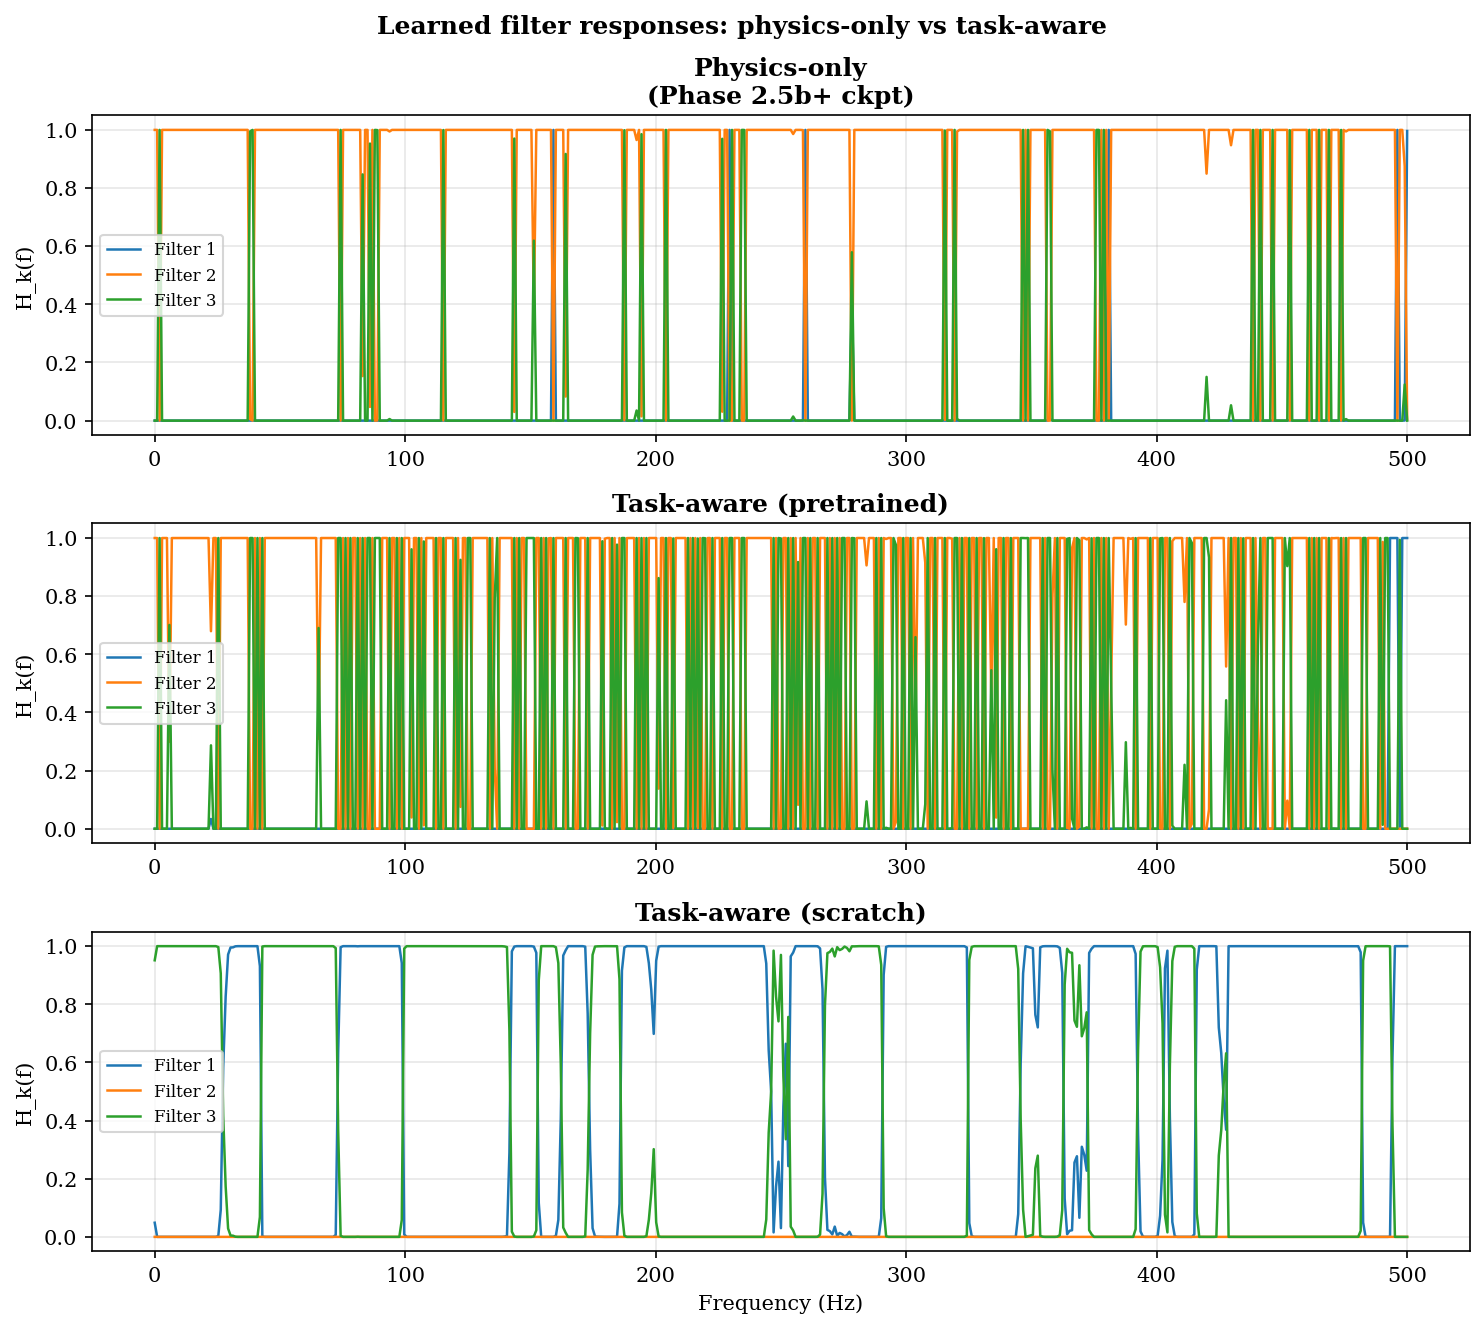
\includegraphics[width=0.9\textwidth]{figures/phase3_exp3/filter_responses.png}
\caption{Learned filter responses under three training regimes on a sample test signal. Task gradients produce sharper filters aligned with class-discriminative frequency bands.}
\label{fig:filter-responses}
\end{figure*}

\paragraph{Robustness across noise levels.} We repeat the same experiment at SNR $\in \{3, 10, 20\}$ dB. Table~\ref{tab:snr-sweep} shows the results. The task-aware advantage is \emph{noise-regime-dependent}: at $3$~dB, N-EMD (scratch) outperforms VMD+MLP by $+7.8$~pp; at $10$~dB the gap inverts to $-7.8$~pp; at $20$~dB it widens to $-17.5$~pp. The pattern is interpretable. At low SNR, VMD's per-signal ADMM produces a degraded decomposition and the downstream MLP cannot compensate; N-EMD's end-to-end training adapts the filter bank to the noisy regime and recovers task-relevant structure that VMD misses. At high SNR, VMD produces clean features with no task-specific tuning, and N-EMD's weaker mode separation (its acknowledged limitation) becomes the bottleneck.

The practical implication: N-EMD's task-aware training is most valuable exactly where it is most needed --- in noisy, challenging operating conditions. In clean-signal regimes, fixed VMD preprocessing is sufficient.

\begin{table}[t]
\centering
\caption{SNR sweep: task-aware classification accuracy. N-EMD wins at low SNR but loses at high SNR.}
\label{tab:snr-sweep}
\begin{tabular}{rllr}
\toprule
SNR & Pipeline & Test acc. & Macro F1 \\
\midrule
$3$ dB  & Raw CNN              & $0.9917$ & $0.9917$ \\
        & EMD + MLP            & $0.8083$ & $0.8075$ \\
        & VMD + MLP            & $0.8700$ & $0.8707$ \\
        & N-EMD pre.\ + MLP    & $0.8950$ & $0.8940$ \\
        & N-EMD scratch (e2e)  & $\mathbf{0.9483}$ & $\mathbf{0.9484}$ \\
\midrule
$10$ dB & Raw CNN              & $0.9983$ & $0.9983$ \\
        & EMD + MLP            & $0.8417$ & $0.8393$ \\
        & VMD + MLP            & $\mathbf{0.9383}$ & $\mathbf{0.9380}$ \\
        & N-EMD pre.\ + MLP    & $0.7200$ & $0.6555$ \\
        & N-EMD scratch (e2e)  & $0.8600$ & $0.8589$ \\
\midrule
$20$ dB & Raw CNN              & $0.9967$ & $0.9967$ \\
        & EMD + MLP            & $0.9233$ & $0.9232$ \\
        & VMD + MLP            & $\mathbf{0.9533}$ & $\mathbf{0.9533}$ \\
        & N-EMD pre.\ + MLP    & $0.7183$ & $0.7073$ \\
        & N-EMD scratch (e2e)  & $0.7783$ & $0.7781$ \\
\bottomrule
\end{tabular}
\end{table}

%======================================================================
\section{Discussion and Limitations}
\label{sec:discussion}
%======================================================================

\textbf{Mode-mixing gap.} On the pure decomposition task (Section~\ref{sec:generalization}), VMD outperforms N-EMD on mode mixing by $0.1$--$0.2$ points across distributions. We do not hide this. Our claim is not that N-EMD is the best unsupervised decomposition method; it is that N-EMD is the first differentiable decomposition with provable architectural guarantees, and that its differentiability yields downstream advantages (Section~\ref{sec:task-aware}) that fixed methods cannot match. Mode mixing measured per se is the wrong success metric when the decomposition serves a task.

\textbf{Fixed $K$.} Our architecture requires specifying the number of IMFs $K$ at training time. EMD adaptively chooses $K$ per signal; our filter bank does not. The $K$-mismatch experiment (set E in Table~\ref{tab:generalization}) shows that the method degrades gracefully when the true number of components exceeds $K$, but adaptive $K$ is clearly valuable. An obvious extension is a learned stopping criterion on the filter-bank output.

\textbf{Frequency-domain only.} Our analyzer operates on the full-signal spectrum. For long nonstationary signals (minutes of EEG, hours of seismology) where components appear and disappear over time, a joint time-frequency analyzer (e.g., short-time FFT input) would be more appropriate.

\textbf{One dataset.} The task-aware benchmark in Section~\ref{sec:task-aware} is synthetic. The amplitude-in-band structure is deliberately designed to be friendly to frequency-domain decomposition; a classifier using N-EMD features should do well. We report a positive result under favorable conditions; extension to a real-world benchmark (e.g., PhysioNet ECG records, Case Western Reserve bearing faults) is the immediate next step.

%======================================================================
\section{Conclusion}
\label{sec:conclusion}
%======================================================================

We introduced N-EMD, a differentiable signal decomposition built around a softmax partition-of-unity over $K$ learned bandpass filters. The architecture provides exact reconstruction, a Parseval bound on component energy, and approximate orthogonality, all as structural consequences rather than empirical outcomes. End-to-end training with a downstream task improves classification accuracy by $7.8$ percentage points over VMD+classifier on a controlled benchmark. Along the way we documented a negative result: a generic iterative sifting network trained with seven soft physics losses cannot escape degenerate solutions, because soft constraints do not shrink the feasible set.

The practical story is simple. If one needs a \emph{fixed interpretable} decomposition, classical methods are fine; VMD slightly outperforms our method on raw mode-mixing metrics. If one needs a \emph{task-adaptive interpretable} decomposition --- that is, a decomposition that is both physically meaningful and trainable with the task --- this has not previously been possible with classical methods or with black-box neural networks. N-EMD occupies that gap.

%======================================================================
\section*{Reproducibility}
%======================================================================

Code, scripts, and trained checkpoints are available at
\url{https://github.com/<pending>}. All experiments run on CPU; no GPU is required. The full library is $2{,}939$ lines of Python; the experiment scripts are $2{,}602$ lines; test suite $1{,}170$ lines, $125$ tests passing. The filter-bank model has $125{,}315$ trainable parameters. Phase 2.5b+ training takes $\sim 45$ minutes on 6 CPU cores for $100$ epochs; the task-aware run (Table~\ref{tab:task-aware-3db}) takes $\sim 1.75$ hours for $50$ end-to-end epochs.

%======================================================================
\bibliographystyle{IEEEtran}
\bibliography{references}
%======================================================================

\end{document}
